\subsection{Preventivo fase di sviluppo}

\subsubsection{Divisione oraria}
La seguente tabella rappresenta la distribuzione oraria dei ruoli per ogni componente del gruppo:
{
	\rowcolors{2}{\evenRowColor}{\oddRowColor}
	\renewcommand{\arraystretch}{2}
	\begin{longtable}[h!] { C{3.5cm} C{1cm} C{1cm} C{1cm} C{1cm} C{1cm} C{1cm} C{2cm}}
	\caption{Tabella della divisione oraria fase di Sviluppo}\\
	\rowcolor{\primaryColor}
	
	\textcolor{\secondaryColor}{\textbf{Membro del gruppo}} & 
	\textcolor{\secondaryColor}{\textbf{RE}} & 
	\textcolor{\secondaryColor}{\textbf{AM}} & 
	\textcolor{\secondaryColor}{\textbf{AN}} & 
	\textcolor{\secondaryColor}{\textbf{PT}} & 
	\textcolor{\secondaryColor}{\textbf{PR}} & 
	\textcolor{\secondaryColor}{\textbf{VE}} & 
	\textcolor{\secondaryColor}{\textbf{Ore complessive}}\\	
	\endhead
	
	\AW{}                     & - & - & - & 12 & 19 & 17 & 48 \\
	\AT{}                     & 11 & - & - & 10 & 15 & 13 & 49 \\
	\AD{}                     & 10 & - & - & 7 & 18 & 14 & 49 \\
	\EC{}                     & - & - & - & 13 & 18 & 17 & 48 \\
	\EM{}                     & - & 8 & - & 10 & 19 & 11 & 48 \\
	\FP{}                     & - & 8 & - & 11 & 18 & 12 & 49 \\
	\GG{}                     & - & 8 & - & 10 & 19 & 12 & 49 \\
	\textbf{Ore totali ruolo} & 21 & 24 & - & 73 & 126 & 96 & 340\\
	
	\end{longtable}
}

% Responsabile color=blue, Amministratore color=yellow, Analista color=red, Progettista color=green, Programmatore color=grigetto, Verificatore color=orange  [ybar, fill=] blue, yellow, red, green, grigetto, orange

\begin{figure}[h!]
	\caption{Istogramma relativo alla suddivisione delle ore preventivate per ciascun componente del gruppo e per ogni ruolo nella fase di sviluppo}
    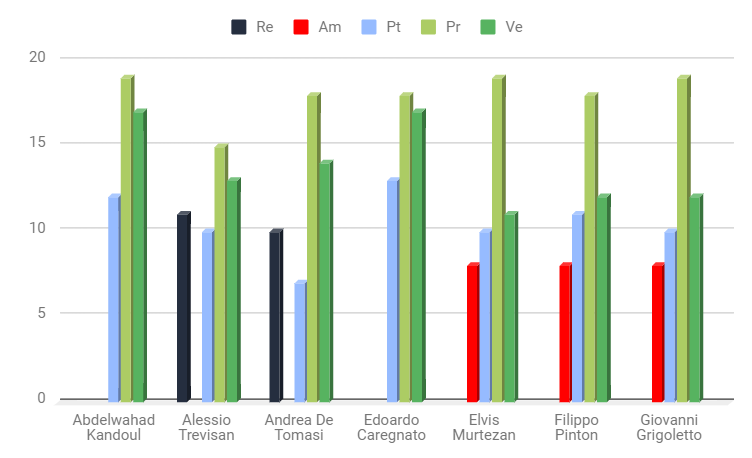
\includegraphics[width=1\textwidth]{./src/Preventivo/src/img/IstoSviluppo.png}  
\end{figure}

%\begin{center}
%	\pgfplotsset{width=15.4cm, height=8.5cm}
%	\begin{tikzpicture}
%		\begin{axis}[
%			ybar stacked,
%			bar width=20pt,
%			legend style={
%				at={(0.5,-0.15)},
%				anchor=north,
%				legend columns=-1
%			},
%			symbolic x coords={Abdelwahad, Alessio, Andrea, Edoardo, Elvis, Filippo, Giovanni},
%			xtick=data
%		]
%			\legend{Responsabile, Amministratore, Analista, Progettista, Programmatore, Verificatore}
			% Responsabile
%			\addplot [ybar, fill=blue] coordinates {\ColonnaIstogramma{0}{11}{10}{0}{0}{0}{0}};
			% Amministratore
%			\addplot [ybar, fill=yellow] coordinates {\ColonnaIstogramma{0}{0}{0}{0}{8}{8}{8}};
			% Analista
%			\addplot [ybar, fill=red] coordinates {\ColonnaIstogramma{0}{0}{0}{0}{0}{0}{0}};
			% Progettista
%			\addplot [ybar, fill=green] coordinates {\ColonnaIstogramma{12}{10}{7}{13}{10}{11}{10}};
			% Programmatore
%			\addplot [ybar, fill=pink] coordinates {\ColonnaIstogramma{19}{15}{18}{18}{19}{18}{19}};
			% Verificatore
%			\addplot [ybar, fill=orange] coordinates {\ColonnaIstogramma{17}{13}{14}{17}{11}{12}{12}};
%		\end{axis}
%	\end{tikzpicture}
%\end{center}
\clearpage
% \subsubsection{Ore e costi degli incrementi}
% La seguente tabella rappresenta la distribuzione delle ore investite durante il periodo in cui vengono svolti gli incrementi e il corrispondente costo in euro.


% {
% \rowcolors{2}{\evenRowColor}{\oddRowColor}
% \renewcommand{\arraystretch}{1.65}
% \centering
% \begin{longtable}{ C{2.1cm} C{2.7cm} C{3cm} C{3cm} C{3.3cm} }
% \caption{Tabella del costo risultante di ogni incremento}\\
% \rowcolor{\primaryColor}
% \textcolor{\secondaryColor}{\textbf{Incremento}} & 
% \textcolor{\secondaryColor}{\textbf{Ore progettista}} &
% \textcolor{\secondaryColor}{\textbf{Ore programmatore}}&
% \textcolor{\secondaryColor}{\textbf{Ore verificatore}}&
% \textcolor{\secondaryColor}{\textbf{Costo totale incremento (in \euro{})}}\\
% \endhead


% x & x & x & x & x\\
% x & x & x & x & x\\
% x & x & x & x & x\\
% x & x & x & x & x\\
% x & x & x & x & x\\



% \end{longtable}
% }


\subsubsection{Costo risultante}
La seguente tabella rappresenta, per ruolo, le ore preventivate totali ed il corrispondente costo in euro:
{
\rowcolors{2}{\evenRowColor}{\oddRowColor}
\renewcommand{\arraystretch}{2}
\begin{longtable}{ C{3cm} C{2cm} C{4cm}}
\caption{Tabella del costo risultante di Sviluppo}\\
\rowcolor{\primaryColor}

\textcolor{\secondaryColor}{\textbf{Ruolo}} & 
\textcolor{\secondaryColor}{\textbf{Totale ore}} & 
\textcolor{\secondaryColor}{\textbf{Costo ruolo (in \euro{})}}\\	
\endhead
        
Responsabile    & 21 & 630 \\
Amministratore  & 24 & 480 \\
Analista        & - & - \\
Progettista     & 73 & 1606 \\
Programmatore   & 126 & 1890 \\
Verificatore    & 96 & 1440 \\
\textbf{Totale} & 340 & 6046 \\
		
\end{longtable}
}



\begin{figure}[h!]
	\caption{Areogramma relativo alla quantità di ore totali preventivate per ciascun ruolo nella fase di sviluppo}
    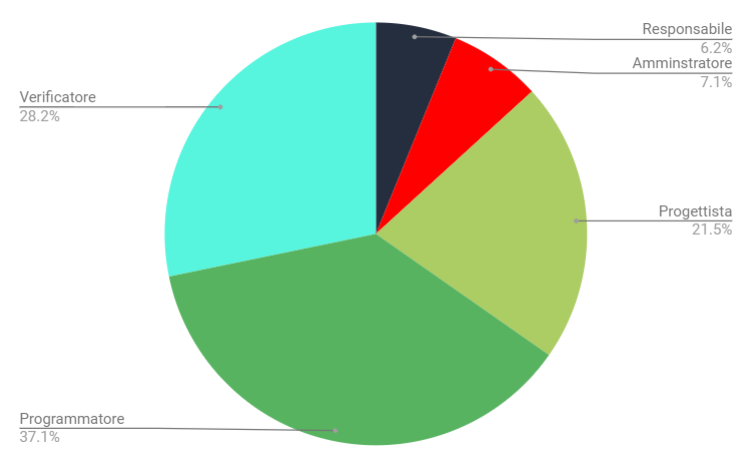
\includegraphics[width=1\textwidth]{./src/Preventivo/src/img/TortaSviluppo.png}  
\end{figure}

%\begin{center}
%	\begin{tikzpicture}
%		\pie[rotate = 180, color={blue, yellow, green, pink, orange}] {
%			6/Responsabile,
%			7/Amministratore,
%			22/Progettista,
%			37/Programmatore,
%			28/Verificatore
%		}
%	\end{tikzpicture}
%\end{center}